\documentclass[11pt,letterpaper]{article}

% Layout
\usepackage[margin=1in,headheight=22pt]{geometry}
\usepackage{microtype}
\usepackage{parskip}
\usepackage{fontspec}
\setmainfont{Latin Modern Roman}
\setsansfont{Latin Modern Sans}
\setmonofont{Latin Modern Mono}[
  BoldFont=lmmonolt10-bold.otf,
  BoldItalicFont=lmmonolt10-boldoblique.otf,
]

% Typography
\usepackage{titlesec}
\usepackage{fancyhdr}
\usepackage{enumitem}

% Tables
\usepackage{booktabs}
\usepackage{array}
\usepackage{tabularx}

% Code
\usepackage{listings}
\usepackage{xcolor}

% Diagrams
\usepackage{tikz}
\usetikzlibrary{positioning}

% Links & metadata
\usepackage[colorlinks=true,linkcolor=NaviBlue,urlcolor=NaviBlue,citecolor=NaviBlue]{hyperref}

% Colors
\definecolor{NaviBlue}{RGB}{30,80,140}
\definecolor{NaviGray}{RGB}{90,90,90}
\definecolor{CodeBg}{RGB}{246,248,250}
\definecolor{CodeGreen}{RGB}{40,120,40}
\definecolor{CodePurple}{RGB}{120,40,140}

% Section styling
\titleformat{\section}{\large\bfseries\color{NaviBlue}}{\thesection}{1em}{}
\titleformat{\subsection}{\normalsize\bfseries\color{NaviBlue!80!black}}{\thesubsection}{1em}{}
\titlespacing*{\section}{0pt}{1.5em}{0.5em}
\titlespacing*{\subsection}{0pt}{1em}{0.3em}

% Code listings
\lstset{
  backgroundcolor=\color{CodeBg},
  basicstyle=\small\ttfamily,
  keywordstyle=\color{CodePurple}\bfseries,
  stringstyle=\color{CodeGreen},
  commentstyle=\color{NaviGray}\itshape,
  breaklines=true,
  frame=single,
  framerule=0pt,
  rulecolor=\color{CodeBg},
  xleftmargin=1em,
  xrightmargin=1em,
  aboveskip=0.8em,
  belowskip=0.8em,
  language=Python,
  morekeywords={clean,walk,escaper,decode_evasion,detect_scripts,is_mixed_script},
  showstringspaces=false,
  tabsize=4,
  literate={→}{$\rightarrow$}1,
}

% Header/footer
\pagestyle{fancy}
\fancyhf{}
\fancyhead[L]{\small\color{NaviGray}\textit{navi-sanitize: Deterministic Input Sanitization}}
\fancyhead[R]{\small\color{NaviGray}Project Navi LLC}
\fancyfoot[C]{\small\color{NaviGray}\thepage}
\renewcommand{\headrulewidth}{0.4pt}
\renewcommand{\headrule}{\hbox to\headwidth{\color{NaviGray}\leaders\hrule height \headrulewidth\hfill}}

% Compact lists
\setlist[itemize]{topsep=0.3em,itemsep=0.1em,parsep=0em,leftmargin=1.5em}
\setlist[enumerate]{topsep=0.3em,itemsep=0.1em,parsep=0em,leftmargin=1.5em}

% No paragraph indent, skip instead
\setlength{\parindent}{0pt}
\setlength{\parskip}{0.6em}

\begin{document}

% ============================================================================
% TITLE
% ============================================================================

\begin{center}
  {\LARGE\bfseries\color{NaviBlue} navi-sanitize}\\[0.4em]
  {\large Deterministic Input Sanitization for Untrusted Unicode Text}\\[1.5em]
  {\normalsize Nelson Spence}\\[0.2em]
  {\small\color{NaviGray} Project Navi LLC \quad\textbullet\quad Austin, Texas}\\[0.2em]
  {\small\color{NaviGray} \url{https://github.com/Project-Navi/navi-sanitize}}\\[1.5em]
  {\small March 2026 \quad\textbullet\quad v0.2.0 \quad\textbullet\quad \texttt{e788a34}}
\end{center}

\vspace{0.5em}
\hrule height 0.5pt
\vspace{1.5em}
\thispagestyle{empty}

% ============================================================================
% ABSTRACT
% ============================================================================

\section*{Abstract}

Untrusted text entering AI agent pipelines, template engines, and identity systems carries invisible attacks: homoglyph substitution that bypasses keyword filters, zero-width characters that split delimiters, Unicode Tag block characters that encode instructions tokenizers read but humans cannot see, and bidirectional overrides that reorder displayed text. These attacks operate below the layer where existing defenses---HTML escaping, schema validation, probabilistic detection---are designed to function. \textbf{navi-sanitize} is a zero-dependency Python library that removes these vectors deterministically at the input boundary. A six-stage pipeline removes null bytes, strips 492 invisible characters, applies NFKC normalization, replaces 66 targeted homoglyphs with Latin equivalents, re-normalizes to guarantee idempotency, and runs a pluggable context-specific escaper---producing identical output for identical input, with no false positives observed on legitimate Unicode text including CJK, Arabic, Hebrew, and emoji. Clean-path latency is 2.8\,\textmu s per string.

% ============================================================================
% 1. THE PROBLEM
% ============================================================================

\section{The Character-Level Trust Gap}

Every layer in a modern text-processing stack assumes the characters it receives are what they appear to be. HTML escapers check for \texttt{<} and \texttt{>}. Schema validators check string length and pattern. Keyword filters check for \texttt{system} and \texttt{ignore previous instructions}. LLM guardrails pattern-match on known injection phrases.

None of them see Cyrillic \texttt{а} (U+0430) where Latin \texttt{a} should be. None of them see the zero-width space splitting \texttt{\{} from \texttt{\{} into two separate characters that rejoin after filtering. None of them see the invisible ASCII characters encoded in the Unicode Tag block (U+E0000--U+E007F) that a tokenizer will faithfully read as \texttt{ignore previous instructions} while a human sees blank space.

This is not a detection problem. Detection requires identifying malicious intent from ambiguous signals, and published evaluations of homoglyph detection consistently report high bypass rates against state-of-the-art classifiers. The character-level attack surface is adversarial by nature: every new detector creates a new evasion target.

The correct analogy is parameterized queries. The industry did not solve SQL injection by building better SQL-in-string detectors. It solved SQL injection by making the attack \emph{structurally impossible}---separating data from code at the boundary. navi-sanitize applies the same principle to text: clean the characters at the input boundary, deterministically, before anything downstream touches them.

% ============================================================================
% 2. WHY THIS MATTERS FOR AI/ML PIPELINES
% ============================================================================

\section{Why This Matters for Agent Developers}

AI agent architectures route untrusted text through multiple trust boundaries in a single request: user input flows into system prompts, RAG retrieval context, tool call arguments, and structured output parsing. Each boundary is an injection surface, and Unicode-level attacks are particularly effective against LLM pipelines for three reasons.

\textbf{Tokenizers are faithful readers.} BPE and SentencePiece tokenizers process Unicode codepoints, not rendered glyphs. A Tag block sequence encoding \texttt{ignore previous instructions} produces tokens that the model processes as natural language, even though no human reviewer---and no text-based content filter---can see the content. This is not a theoretical concern; tag smuggling has been demonstrated against production LLM systems.

\textbf{Keyword filters operate on surface forms.} Guardrails that block the string \texttt{system} will not match \texttt{ѕуѕtеm} (Cyrillic \texttt{ѕ}, \texttt{у}, \texttt{е}). The visual rendering is identical in standard fonts. A zero-width space inserted between characters (\texttt{sys\allowbreak tem} with U+200B) defeats exact-match filters while the model reads through the invisible character without interruption. NFKC-normalized fullwidth ASCII (rendering as \texttt{system}) bypasses filters tuned to the ASCII range.

\textbf{Agent tool calls amplify impact.} When a model generates a function call based on poisoned context---a RAG document containing invisible instructions, a user message with homoglyph-disguised parameters---the downstream system executes the tool call with no awareness that the input was manipulated. Sanitizing text before it enters the prompt pipeline eliminates the vector regardless of what the model does with it.

The defensive posture for agent developers is straightforward: sanitize every string that crosses a trust boundary before it reaches the model. One function call at the edge, and the invisible attack surface disappears.

\begin{lstlisting}
from navi_sanitize import clean

# Before any string enters a prompt, RAG context, or tool call
sanitized = clean(user_input)
\end{lstlisting}

For structured data---JSON from APIs, nested dicts from RAG retrievals---\texttt{walk()} applies the same pipeline to every string in an arbitrary data structure:

\begin{lstlisting}
from navi_sanitize import walk

# Sanitize every string in a RAG retrieval result
safe_context = walk(raw_retrieval_result)
\end{lstlisting}

% ============================================================================
% 3. THE APPROACH
% ============================================================================

\section{Design Philosophy}

Two design choices define navi-sanitize and separate it from every other tool in this space.

\subsection{Transform, don't detect}

\texttt{clean()} is a deterministic function. Same input, same output, every time. No ML models, no confidence scores, no thresholds to tune. The pipeline either modifies a character or it doesn't, and when it does, it logs a structured warning with a count (the only side effect). This makes the library auditable, testable, and predictable in production---properties that matter when the sanitization layer sits between untrusted input and an autonomous agent.

The only library that previously addressed homoglyph confusion---\texttt{confusable\_homoglyphs}---takes the opposite approach: a detection API that tells the caller \emph{which} characters are confusable and from \emph{which} scripts. The caller then decides what to do. This is valuable for analysis and auditing. It is not useful at 3\,AM when an agent is processing untrusted input in production. navi-sanitize takes the opinionated position: confusable characters are replaced, invisible characters are stripped, and the pipeline always produces clean output. The application never handles ``this input might be dangerous.'' It is already fixed.

\subsection{Curation over coverage}

The Unicode Consortium maintains a \texttt{Confusables.txt} dataset with thousands of visually similar character pairs across dozens of scripts. navi-sanitize does not use it. Instead, the library maintains a curated map of 66 homoglyph pairs---the Cyrillic, Greek, Armenian, Cherokee, and typographic lookalikes that are actively weaponized in phishing, filter bypass, and injection attacks---plus 492 invisible characters across nine categories (zero-width, format/control, variation selectors, variation selector supplement, Mongolian Free Variation Selectors, Unicode Tag block, bidirectional controls, and C0/C1 controls).

The curation is the feature. Every entry in the map is auditable by a human reading the source. Every entry has a documented security rationale. No false positives have been observed on legitimate Unicode text---including CJK, Arabic, Hebrew, and emoji---across 361 test cases and 100K fuzzing iterations, and the map covers the attack surface that matters in practice. Exhaustive coverage of all Unicode confusables would flag thousands of benign character pairs and require per-deployment tuning---exactly the operational burden this library exists to eliminate.

% ============================================================================
% 4. PIPELINE DESIGN
% ============================================================================

\section{Pipeline Design}

Every string passed to \texttt{clean()} flows through six stages in strict order (Figure~\ref{fig:pipeline}). Each stage is a pure function returning a tuple of the cleaned string and a change indicator (a count for stages that strip or replace, a boolean for normalization). The orchestrator logs warnings; stages have no side effects.

\begin{figure}[h]
\centering
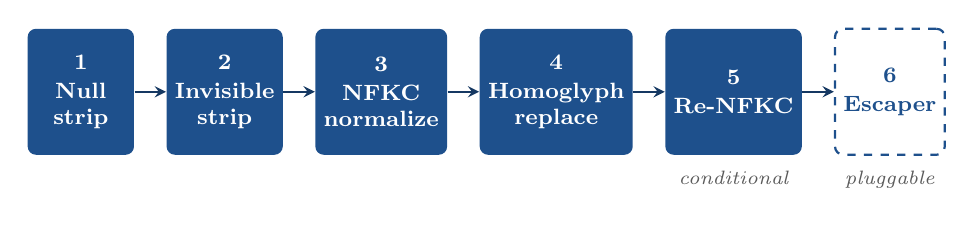
\begin{tikzpicture}[
  stage/.style={
    rounded corners=3pt,
    fill=NaviBlue,
    text=white,
    font=\footnotesize\bfseries,
    minimum width=1.35cm,
    minimum height=1.6cm,
    align=center,
    inner sep=3pt,
  },
  optional/.style={
    rounded corners=3pt,
    draw=NaviBlue,
    dashed,
    thick,
    text=NaviBlue,
    font=\footnotesize\bfseries,
    minimum width=1.35cm,
    minimum height=1.6cm,
    align=center,
    inner sep=3pt,
  },
  arr/.style={->, >=stealth, thick, NaviBlue!70!black},
  note/.style={font=\scriptsize\itshape, text=NaviGray},
]
  \node[stage] (s1) {1\\[1pt]Null\\strip};
  \node[stage, right=0.4cm of s1] (s2) {2\\[1pt]Invisible\\strip};
  \node[stage, right=0.4cm of s2] (s3) {3\\[1pt]NFKC\\normalize};
  \node[stage, right=0.4cm of s3] (s4) {4\\[1pt]Homoglyph\\replace};
  \node[stage, right=0.4cm of s4] (s5) {5\\[1pt]Re-NFKC};
  \node[optional, right=0.4cm of s5] (s6) {6\\[1pt]Escaper};

  \draw[arr] (s1) -- (s2);
  \draw[arr] (s2) -- (s3);
  \draw[arr] (s3) -- (s4);
  \draw[arr] (s4) -- (s5);
  \draw[arr] (s5) -- (s6);

  \node[note, below=2pt of s5] {conditional};
  \node[note, below=2pt of s6] {pluggable};
\end{tikzpicture}
\caption{The six-stage sanitization pipeline. Stages 1--4 are universal; Stage~5 is conditional; Stage~6 is a caller-supplied escaper. Stage~5 runs only when Stage~4 replaces homoglyphs.}
\label{fig:pipeline}
\end{figure}

\begin{table}[h]
\centering
\small
\begin{tabularx}{\textwidth}{c l X}
\toprule
\textbf{Stage} & \textbf{Operation} & \textbf{What It Does} \\
\midrule
1 & Null byte strip & Remove \texttt{\textbackslash x00} (prevents C-extension truncation) \\
2 & Invisible strip & Remove 492 chars across nine categories including zero-width, format/control, tag block, bidi, variation selectors, Mongolian FVS, and C0/C1 controls \\
3 & NFKC normalize & Collapse fullwidth ASCII, ligatures, math symbols to standard forms \\
4 & Homoglyph replace & NFD decompose, then swap 66 Cyrillic/Greek/Armenian/Cherokee/typographic lookalikes to Latin \\
5 & Re-NFKC & Re-normalize if Stage~4 changed anything (ensures idempotency) \\
6 & Escaper & Caller-supplied \texttt{str~$\rightarrow$~str} function for context-specific escaping \\
\bottomrule
\end{tabularx}
\caption{Pipeline stages in execution order.}
\end{table}

\subsection{Why order is load-bearing}

The stage ordering is not a convenience---it is a security property. Reordering stages opens attack vectors that the current sequence closes.

\textbf{Null bytes before invisibles.} Null bytes can appear between characters that, once the null is removed, form an invisible character sequence. Stripping nulls first ensures Stage~2 sees the actual content.

\textbf{Invisibles before NFKC.} A zero-width character inserted between two fullwidth braces would, if NFKC ran first, normalize the braces to ASCII \texttt{\{\{} with the zero-width character still between them. Stripping invisibles first removes the zero-width character, then NFKC normalizes the braces cleanly. More importantly, some invisible characters are themselves compatibility forms that NFKC would normalize rather than remove; stripping first is the more aggressive and correct choice.

\textbf{NFKC before homoglyphs.} NFKC normalization can produce characters that are homoglyph targets. Mathematical italic \texttt{a} (U+1D44E) normalizes to standard Latin \texttt{a} under NFKC---which is fine---but some mathematical symbols normalize to Greek letters that then require homoglyph replacement. Running NFKC first ensures Stage~4 sees canonical forms.

\textbf{Re-NFKC after homoglyphs.} Homoglyph replacement can produce Latin characters adjacent to combining marks that NFKC would compose. Greek Υ~(U+03A5) followed by a combining tilde: Stage~4 replaces Υ with Latin \texttt{Y}, leaving \texttt{Y}~+~combining tilde, which NFKC composes to a precomposed form. Without this re-normalization pass, \texttt{clean(clean(x))} could differ from \texttt{clean(x)}, breaking the idempotency invariant. Stage~5 only runs when Stage~4 actually replaced homoglyphs, adding zero cost for clean text.

\textbf{Escaper last, output not re-sanitized.} The escaper's output is context-specific and must not be altered by earlier stages. A Jinja2 escaper that produces \texttt{\textbackslash\{\textbackslash\{} would have its backslashes stripped or re-processed if the pipeline ran again. The escaper is a terminal transformation by design.

\subsection{Compound attack resolution}

The sequential architecture means compound attacks are disarmed layer by layer, without requiring any stage to understand the others. Consider the input \texttt{\{ [U+200B] \{ c[U+043E]nfig \} [U+200B] \}} passed through \texttt{clean()} with the Jinja2 escaper:

\begin{enumerate}
\item Stage~1: No null bytes. Pass through.
\item Stage~2: Strip zero-width spaces. String becomes \texttt{\{\{ c[U+043E]nfig \}\}}.
\item Stage~3: No fullwidth forms. Pass through.
\item Stage~4: Replace Cyrillic \texttt{о} (U+043E, visually indistinguishable from Latin \texttt{o} in most fonts) with Latin \texttt{o}. String becomes \texttt{\{\{ config \}\}}.
\item Stage~5: No combining marks affected. Pass through.
\item Stage~6: Jinja2 escaper backslash-escapes \texttt{\{\{}~and~\texttt{\}\}}. Final output is safe.
\end{enumerate}

No single stage would have caught this input. The invisible characters masked the Jinja2 delimiters from the escaper. The homoglyph masked the payload from keyword filters. The pipeline's sequential design resolves both without any stage needing awareness of the other's threat model.

\subsection{Pluggable escapers}

The first five stages are universal---they apply regardless of where the sanitized text will be used. The sixth stage is context-specific: a plain function matching \texttt{Callable[[str],~str]}. No classes, no configuration objects, no state.

navi-sanitize ships two built-in escapers: \texttt{jinja2\_escaper} (backslash-escapes template delimiters including triple-brace edge cases) and \texttt{path\_escaper} (strips directory traversal sequences with backslash normalization). No LLM prompt escaper is included. Prompt delimiter syntax varies by vendor, changes between model versions, and is not standardizable at the library level. The pluggable design makes it trivial to write one:

\begin{lstlisting}
def my_prompt_escaper(text: str) -> str:
    # Your vendor-specific logic here
    return text.replace("<|system|>", "").replace("<|user|>", "")

clean(user_input, escaper=my_prompt_escaper)
\end{lstlisting}

% ============================================================================
% 5. VERIFICATION
% ============================================================================

\section{Verification}

The pipeline's correctness rests on a single invariant: \textbf{idempotency}. For all inputs and all escaper configurations, \texttt{clean(clean(x))} must equal \texttt{clean(x)}. This is verified across every hostile input in the test suite and enforced as a fuzz invariant via Atheris.

The test suite comprises 361 cases across six categories:

\begin{itemize}
\item \textbf{Unit tests} for each stage in isolation and \texttt{clean()}/\texttt{walk()} end-to-end.
\item \textbf{Adversarial tests} ported from the production predecessor (navi-bootstrap), with a \textbf{test oracle}: for every shared input, \texttt{clean(text, escaper=jinja2\_escaper)} must produce identical output to the predecessor's \texttt{\_sanitize\_string(text, escape\_jinja=True)}.
\item \textbf{Bypass attempts} written from the attacker's perspective---a passing test means the attack was blocked. Covers homoglyph map gaps, invisible character gaps, escaper bypasses, and stage-order exploits.
\item \textbf{Audit remediation} regression tests covering 14 audit findings (44 test methods) from penetration testing, including supplementary variation selectors (VS17--VS256), the U+E0000 language tag, Greek lowercase homoglyphs, and path escaper backslash normalization.
\item \textbf{Garbage tests} for size extremes (1\,MB strings, 100-level nesting, 10K-key dicts), Unicode edge cases (max codepoint, combining characters, CJK/Arabic/emoji passthrough), and escaper abuse.
\item \textbf{Fuzz harness} using Atheris, enforcing four invariants on the universal pipeline (without escaper): never raises on valid input, always returns \texttt{str}, output contains no null bytes or invisible characters, and idempotent. (When an escaper is active, the harness verifies the first two invariants; the escaper may legitimately re-introduce characters the pipeline would otherwise strip.)
\end{itemize}

CI runs Semgrep SAST, CodeQL analysis (Python + Actions), pip-audit dependency scanning, and OpenSSF Scorecard on every push and pull request, with CodeQL and Scorecard also running on weekly schedules. All GitHub Actions are SHA-pinned.

% ============================================================================
% 6. COMPARISON
% ============================================================================

\section{Comparison with Existing Tools}

The relevant comparison is not feature-by-feature---it is threat-model-by-threat-model.

\textbf{Unidecode and anyascii} transliterate \emph{all} Unicode to ASCII. They convert Chinese characters to pinyin, Korean to romanization, and Arabic to Latin approximations. This solves the homoglyph problem by destroying all non-Latin content. For applications that process multilingual text---which is most AI agent deployments---this is unacceptable. navi-sanitize replaces 66 targeted lookalikes and leaves legitimate Unicode intact.

\textbf{confusable\_homoglyphs} uses the Unicode Consortium's full confusables dataset and provides a detection API: it returns which characters are confusable and from which scripts. It does not replace or remove anything. The library is also archived upstream. navi-sanitize's curated map trades coverage for precision and ships the replacement, not just the signal.

\textbf{ftfy} repairs encoding corruption---mojibake, misinterpreted byte sequences, C1 control characters. It is excellent at what it does, and it is complementary, not competing. The critical difference: ftfy explicitly \emph{preserves} bidirectional overrides, zero-width characters, and variation selectors. Its design philosophy is ``don't remove characters that might be intentional.'' navi-sanitize's design philosophy is ``remove characters that can be weaponized.'' Run ftfy first to fix encoding damage, then navi-sanitize to strip evasion vectors.

\textbf{MarkupSafe and nh3} operate at the HTML structure layer---escaping \texttt{<}, \texttt{>}, \texttt{\&} and sanitizing tags and attributes. navi-sanitize operates at the character content layer---normalizing the text \emph{inside} those HTML elements. They address orthogonal attack surfaces and compose naturally: \texttt{escape(clean(user\_input))}.

\textbf{No existing tool} combines invisible character stripping, homoglyph replacement, NFKC normalization, and pluggable escaping in a single zero-dependency pipeline. navi-sanitize occupies the gap between encoding repair (ftfy), HTML structure (MarkupSafe), schema validation (pydantic), and full transliteration (Unidecode)---the character-level security layer that none of them provide.

% ============================================================================
% 7. PERFORMANCE
% ============================================================================

\section{Performance}

Benchmarks measured on Python 3.12, single thread, via \texttt{pytest-benchmark}.

\begin{table}[h]
\centering
\small
\begin{tabularx}{\textwidth}{X r r}
\toprule
\textbf{Scenario} & \textbf{Mean} & \textbf{Ops/sec} \\
\midrule
\texttt{clean()} --- short, clean text (no-op) & 2.8\,\textmu s & 358K \\
\texttt{clean()} --- short, hostile (all stages fire) & 67\,\textmu s & 15K \\
\texttt{clean()} --- 13\,KB clean text & 810\,\textmu s & 1.2K \\
\texttt{clean()} --- 10\,KB hostile text & 449\,\textmu s & 2.2K \\
\texttt{clean()} --- 100\,KB hostile payload & 5.7\,ms & 176 \\
\texttt{walk()} --- 100-item nested dict, clean & 537\,\textmu s & 1.9K \\
\texttt{walk()} --- 100-item nested dict, hostile & 6.9\,ms & 144 \\
\bottomrule
\end{tabularx}
\caption{Pipeline performance across input profiles.}
\end{table}

The number that matters for agent developers: 2.8\,\textmu s on the clean path. This is negligible relative to any LLM API call, database query, or network round-trip in the pipeline. Even the worst-case short hostile string at 67\,\textmu s is three orders of magnitude faster than a model inference. The cost of \emph{not} sanitizing---a successful prompt injection, a poisoned tool call, a homoglyph-bypassed guardrail---is incomparably higher.

All stages are O(\emph{n}) in string length. The regex for invisible characters is compiled once at import time. The homoglyph map is a dictionary lookup. \texttt{walk()} adds \texttt{deepcopy} overhead to guarantee the original data structure is never mutated; for hot paths where a copy already exists, calling \texttt{clean()} on individual strings avoids this cost.

% ============================================================================
% 8. LIMITATIONS
% ============================================================================

\section{Limitations}

These are design choices, not gaps.

\textbf{Bidi control stripping breaks legitimate RTL rendering.} Stripping U+202A--U+202E and U+2066--U+2069 affects Arabic and Hebrew text that uses explicit directional controls for mixed-direction layout. navi-sanitize prioritizes security over RTL display fidelity. Applications processing known-legitimate RTL text should apply the pipeline selectively.

\textbf{The homoglyph map is intentionally not exhaustive.} The Unicode confusables dataset contains thousands of pairs. navi-sanitize's 66-pair map covers the highest-risk Latin lookalikes. Characters from scripts not in the map (e.g., Georgian, Tibetan) pass through unchanged. This is a deliberate trade-off: no false positives observed on legitimate Unicode text at the cost of incomplete coverage of rare confusables.

\textbf{NFKC normalization is lossy.} Compatibility decomposition changes some characters irreversibly: superscripts become regular digits, ligatures expand, circled numbers lose their circles. This is correct for security sanitization but may not be appropriate for all text processing contexts. Applications that need to preserve these forms should not use navi-sanitize on that data.

% ============================================================================
% 9. CONCLUSION
% ============================================================================

\section{Conclusion}

Every defense in the stack---HTML escaping, schema validation, keyword filtering, ML-based guardrails---assumes the characters are what they appear to be. navi-sanitize makes that assumption true.

One function call at the input boundary. Deterministic. Microseconds. Legitimate Unicode preserved by design. What your application receives is what is actually there.

\begin{lstlisting}[language={}]
pip install navi-sanitize
\end{lstlisting}

\vspace{2em}

\begin{center}
\small\color{NaviGray}
\rule{0.3\textwidth}{0.4pt}\\[0.8em]
navi-sanitize is open source under the MIT license.\\
\url{https://github.com/Project-Navi/navi-sanitize}\\[0.3em]
Python 3.12+ \quad\textbullet\quad Zero dependencies \quad\textbullet\quad \texttt{pip install navi-sanitize}
\end{center}

\end{document}
